


\begin{minipage}{\linewidth}
\center{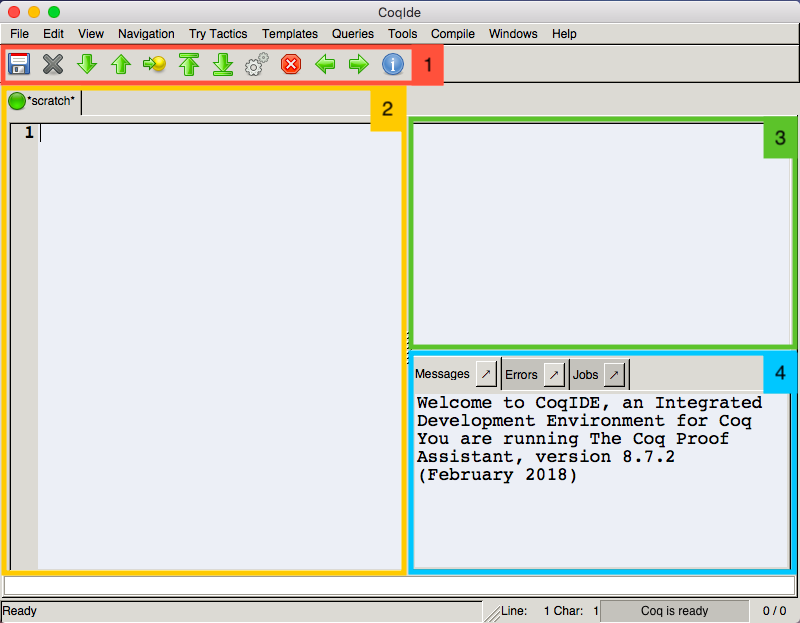
\includegraphics[width=\textwidth]
        {CoqScreenshots/CoqIDE_color.png}}
        \label{fig:IDEcolor} 
        \captionof{figure}{CoqIDE v8.7.2  
        (1) Toolbar. (2) Script Buffer. (3) Goal Window. (4) Message Window. }
\end{minipage}


\subsubsection{Toolbar for CoqIDE v8.7.2}
\hspace{-0.75cm}
\begin{tabular}{ C L }
\centered{
\includegraphics[width=\iconsize]
        {CoqScreenshots/save.png}}
        & \centeredl{Save current buffer. 
        If it hasn't been previously saved, functions as save as; use the extension .v to save as a Coq file.
        } \\ \\
\centered{
\includegraphics[width=\iconsize]
        {CoqScreenshots/close.png}}
	& \centeredl{Close current buffer. 
	Gives a warning if the file has unsaved changes.
	} \\ \\
\centered{
\includegraphics[width=\iconsize]
        {CoqScreenshots/step_forward.png}}
	& \centeredl{Forward one command.
	Steps forward to evaluate the next command in the current file.
	} \\ \\
\centered{
\includegraphics[width=\iconsize]
        {CoqScreenshots/step_backward.png}}
	& \centeredl{Backward one command.
	Steps backward one command in the file, returns the state to where it was before evaluating that command. 
	} \\ \\ 
\centered{
\includegraphics[width=\iconsize]
        {CoqScreenshots/go_to_cursor.png}}
	& \centeredl{Go to cursor.
	Evaluate all commands in file up to where the cursor currently is.
	} \\ \\ 
\centered{
\includegraphics[width=\iconsize]
        {CoqScreenshots/go_to_top.png}}
	& \centeredl{Restart Coq.
	Returns to the top of the file, where no commands have been evaluated.
	} \\ \\ 
\centered{
\includegraphics[width=\iconsize]
        {CoqScreenshots/go_to_bottom.png}}
	& \centeredl{Go to end.
	Evaluate to the bottom of the file. 
	Does not work as well with load commands and require import commands.
	} \\ \\
\centered{
\includegraphics[width=\iconsize]
        {CoqScreenshots/check.png}}
	& \centeredl{Fully check the document.
	Submits proof terms to the Coq kernel for type checking.
	} \\ \\
\centered{
\includegraphics[width=\iconsize]
        {CoqScreenshots/stop.png}}
	& \centeredl{Interrupt computations.
	Stops computation at whatever point was reached before pressing the button.
	} \\ \\
\centered{
\includegraphics[width=\iconsize]
        {CoqScreenshots/next_occurrence.png}}
	& \centeredl{Next Occurrence.
	Goes to the next occurrence of whatever the cursor is currently by. 
	Works well for longer words.
	} \\ \\
\centered{
\includegraphics[width=\iconsize]
        {CoqScreenshots/previous_occurrence.png}}
	& \centeredl{Previous Occurrence.
	Goes to the previous occurrence of whatever the cursor is currently by.
	Works well for longer words.
	} \\ \\
\centered{
\includegraphics[width=\iconsize]
        {CoqScreenshots/proof_wizard.png}}
	& \centeredl{Proof Wizard. 
	Tries to apply a given set of tactics in order. 
	The tactics to be attempted can be customized by going to: 
	Edit tab $\to$ Preferences, then select Tactics Wizard in the leftmost pane of the Customizations window.} 
\end{tabular}






